\section*{Apresentação}

\begin{frame}	
	\begin{block}{Pessoal}	
		\begin{itemize}
			\item Adilson Khouri,  jogador de Magic the Gathering, nerd, apaixonado por computação e machine learning.
		\end{itemize}
		\begin{figure}[!htb]
			\centering	  				
			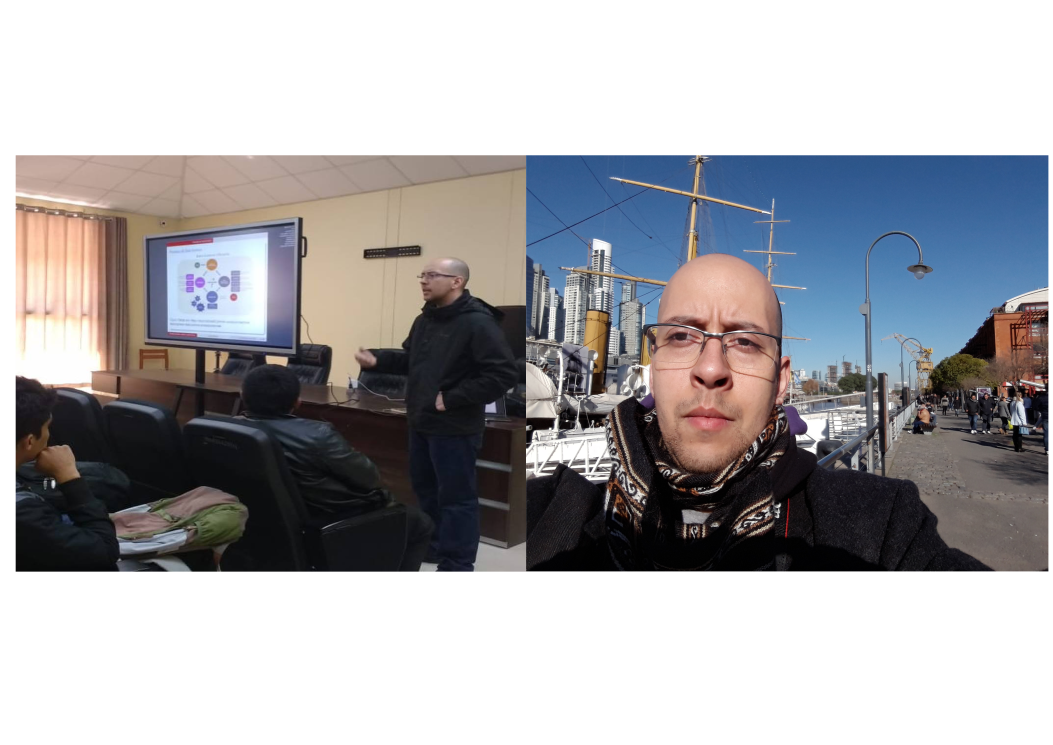
\includegraphics[height=5cm, width = 7cm]{./pic/join.png}
			\caption{Eu no Peru palestrando e na Argentina trabalhando}
			\label{fig_adilson_argentina}
		\end{figure}
		
	\end{block}
\end{frame}
			
\begin{frame}	
	\begin{block}{Formação Acadêmica}
		 \begin{itemize}
			  \item Bacharel em Sistemas de Informação (2011 - USP)
			  \item Mestre em Sistemas de Informação (2016 - USP)
			  \item Doutorando em Sistemas de Informação (cursando - USP)
		  \end{itemize}
	\end{block}
\end{frame}

\begin{frame}	
	\begin{block}{Experiência de Mercado}
		\begin{itemize}
			\item Programador na consultoria Arbit (2010-2011)
			\item Programador Itaú-Unibanco (2011-2013)
			\item Cientista de dados Sr. PagSeguro (2016 - 2018)
			\item Especialista em Modelagem NuvemShop (Atual)
			\item Professor carta convite - SENAC (Atual)
		\end{itemize}
	\end{block}
\end{frame}

\begin{frame}	
	\begin{block}{E os senhores?}
		\begin{itemize}
			\item Nome
			\item Trabalho
			\item Tempo de experiência, área de atuação
			\item Conhecimento sobre o assunto da disciplina
		\end{itemize}
	\end{block}
\end{frame}

\begin{frame}	
	\begin{block}{Expectativas}
		\begin{itemize}
			\item Quais expectativas?
			\item O que deve ser evitado?
			\item (E-Mail: 0800dirso@gmail.com)
		\end{itemize}
	\end{block}
\end{frame}

\begin{frame}	
	\begin{block}{Requisitos}
		\begin{itemize}
			\item Computadores com MAC OS
			\item Computadores com internet
			\item Python, pandas, jupyter notebook, numpy, scipy e scikit-learn
		\end{itemize}
	\end{block}
\end{frame}